\documentclass[peerreview,11pt]{IEEEtran}

% Packages
\usepackage{cite}
\usepackage{graphicx}
\usepackage{subfigure}
\usepackage{float}
\usepackage{url}
\usepackage{color}
\usepackage{amsmath}


\begin{document}

% paper title
% can use linebreaks \\ within to get better formatting as desired
\title{Visual~Perception~Lab~3 \\ Epipolar~Geometry~And~Fundamental~Matrix}
%

\author{Rodrigo~Caye~Daudt}

\definecolor{lightgray}{gray}{0.5}



% make the title area
\maketitle



%%%%%%%%%%%%%%%%%%%%%%%%%%%%%%%%%%%%%%%%%%%%%%%%%%%%%%%%%%%%%%%%%%%%%%%%%%%%%%%
\section{Introduction}

\IEEEPARstart{T}{his} report describes the work done for practical session 3 in the Visual Perception module. In this work we study epipolar geometry, the fundametal matrix, different methods of calculating the fundamental matrix using reference points and the robustness of these methods to different levels of noise using different numbers of points.

All the work described here was developed in MATLAB R2015a for Linux. All the functions and scripts that were written will be delivered alongside this report, and the key lines of code will be quoted in this report as necessary.

%%%%%%%%%%%%%%%%%%%%%%%%%%%%%%%%%%%%%%%%%%%%%%%%%%%%%%%%%%%%%%%%%%%%%%%%%%%%%%%
\section{Part 1}\label{p1}

\subsection{Step 1}

The first step was to define all the necessary parameters relative to camera 1. This camera was assumed to be aligned with the world coordinate system and positioned at its origin. This was done by the following commands:

\begin{verbatim}
% Camera 1 parameters
au1 = 100; av1 = 120; uo1 = 128; vo1 = 128;
sx1 = 256; sy1 = 256;
\end{verbatim}

\subsection{Step 2}

Step 2 consisted of defining all the necessary parameters relative to camera 2. This was done by the following commands:


\begin{verbatim}
% Camera 2 parameters
au2 = 90; av2 = 110; uo2 = 128; vo2 = 128;
ax = 0.1; by = pi/4; cz = 0.2;
tx = -1000; ty = 190; tz = 230;
sx2 = 256; sy2 = 256;
\end{verbatim}


\subsection{Step 3}

In this step the intrinsic transformation matrices of both cameras were calculated, as well as the rotation and translation between the two cameras. This was accomplished by the following commands:

\begin{verbatim}
% Notation: Camera 1 is W and camera 2 is C
% Intrinsic matrices
I1 = [au1 0 uo1; 0 av1 vo1; 0 0 1];
I2 = [au2 0 uo2; 0 av2 vo2; 0 0 1];
% Rotation matrices
Rx = [1 0 0;0 cos(ax) -sin(ax);0 sin(ax) cos(ax)];
Ry = [cos(by) 0 sin(by);0 1 0;-sin(by) 0 cos(by)];
Rz = [cos(cz) -sin(cz) 0;sin(cz) cos(cz) 0;0 0 1];
WRC = Rx*Ry*Rz;
CRW = WRC';
% Translation vectors
T = [tx;ty;tz];
% t_W = -WRC*t_C;
% Transformation matrices
WTC = [WRC, T;0 0 0 1];
CTW = inv(WTC);
\end{verbatim}

\subsection{Step 4}

In this step the correct (ground truth) fundamental matrix between the two defined cameras was calculated using the parameters previously defined using the formula $$F = A'^{-t}R^t [t]_x A^{-1}$$

and the result obtained was 

\[
F = 
\begin{bmatrix}
    0.0000  &  0.0001  & -0.0066\\
    0.0000  & -0.0000  &  0.0130\\
   -0.0096  & -0.0173  &  1.0000\\
\end{bmatrix}
\]

The code used for this operation was:

\begin{verbatim}
t_cross = [0 -T(3) T(2);T(3) 0 -T(1);-T(2) T(1) 0];
F = inv(I2)'*WRC'*t_cross*inv(I1);
F = F/F(3,3);
\end{verbatim}

\subsection{Step 5}


In this step, three sets of points were created with 20, 50 and 150 points to evaluate the behaviour of the algorithms later on. The first 20 points were defined deterministically, while the remaining points were defined randomly in the same ranges for each coordinates. The code used to generate these points was as follows:

\begin{verbatim}
clear V;
V(:,1) = [100;-400;2000;1];
V(:,2) = [300;-400;3000;1];
V(:,3) = [500;-400;4000;1];
V(:,4) = [700;-400;2000;1];
V(:,5) = [900;-400;3000;1];
V(:,6) = [100;-50;4000;1];
V(:,7) = [300;-50;2000;1];
V(:,8) = [500;-50;3000;1];
V(:,9) = [700;-50;4000;1];
V(:,10) = [900;-50;2000;1];
V(:,11) = [100;50;3000;1];
V(:,12) = [300;50;4000;1];
V(:,13) = [500;50;2000;1];
V(:,14) = [700;50;3000;1];
V(:,15) = [900;50;4000;1];
V(:,16) = [100;400;2000;1];
V(:,17) = [300;400;3000;1];
V(:,18) = [500;400;4000;1];
V(:,19) = [700;400;2000;1];
V(:,20) = [900;400;3000;1];

morepoints = [(800*rand(1,30)+100);(800*rand(1,30)-400);
                        (2000*rand(1,30)+200);ones(1,30)];
V50 = [V morepoints];

morepoints = [(800*rand(1,100)+100);(800*rand(1,100)-400);
                        (2000*rand(1,100)+200);ones(1,100)];
V150 = [V50 morepoints];
\end{verbatim}


\subsection{Step 6}

Using the matrix calculated in step 3, the projections onto both cameras of all the points in all three sets of reference points were calculated. In this step, an auxiliary function called \textit{normalise\_scale} was used to normalise the scale of all the projected points to facilitate the operation with these projections from this point on. These operations were performed by the following lines of code:

\begin{verbatim}
A1 = [I1 zeros(3,1)]*[eye(3) zeros(3,1);0 0 0 1];
A2 = [I2 zeros(3,1)]*CTW;

% 20 points
p1 = zeros(3,size(V,2));
p2 = zeros(3,size(V,2));
for i = 1:size(V,2)
    p1(:,i) = A1*V(:,i);
    p2(:,i) = A2*V(:,i);
end
p1 = normalise_scale(p1);
p2 = normalise_scale(p2);

% 50 points
p1_50 = zeros(3,size(V50,2));
p2_50 = zeros(3,size(V50,2));
for i = 1:size(V50,2)
    p1_50(:,i) = A1*V50(:,i);
    p2_50(:,i) = A2*V50(:,i);
end
p1_50 = normalise_scale(p1_50);
p2_50 = normalise_scale(p2_50);

% 150 points
p1_150 = zeros(3,size(V150,2));
p2_150 = zeros(3,size(V150,2));
for i = 1:size(V150,2)
    p1_150(:,i) = A1*V150(:,i);
    p2_150(:,i) = A2*V150(:,i);
end
p1_150 = normalise_scale(p1_150);
p2_150 = normalise_scale(p2_150);
\end{verbatim}

\subsection{Step 7}

In this step we visualised the projections calculated in the previous step. The result were six visualisations, comprising all combinations of camera (1 or 2) and number of reference points (20, 50 or 150). The borders of the camera sensors were also drawn on these plots to serve as references. The resulting drawings can be found in Fig. \ref{fig:refpoints}.

It should be noted here that the points generated after the twentieth point were random, so each run of the code will result in different sets of points and different results.

\begin{figure}[ht]
	\centering

	\subfigure[20 reference points in camera 1 plane]{\label{c1_20}
		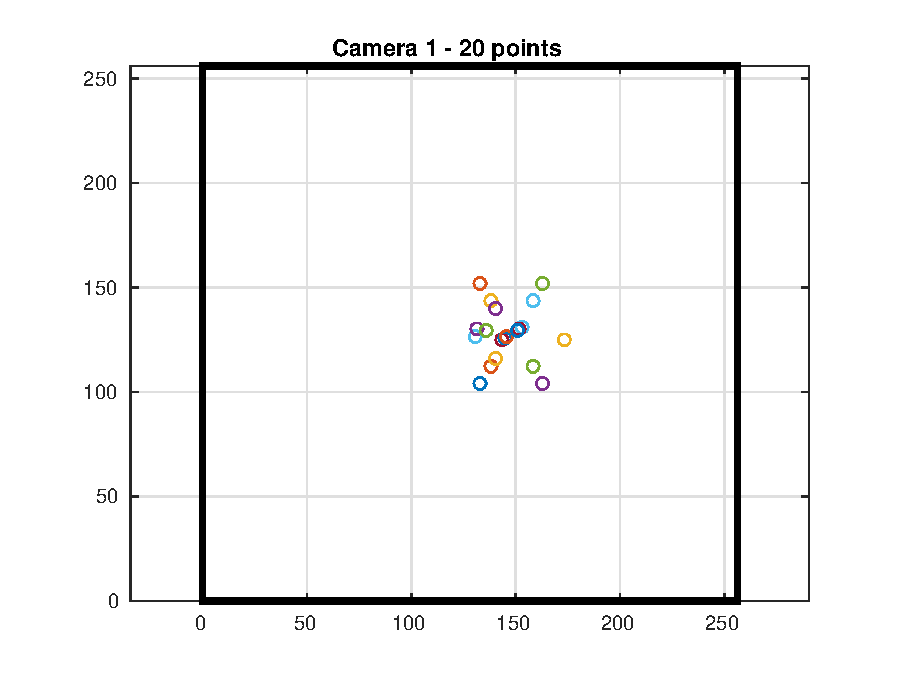
\includegraphics[width=0.4\linewidth]{figures/c1_20.eps}}~
	\subfigure[20 reference points in camera 2 plane]{\label{c2_20}
		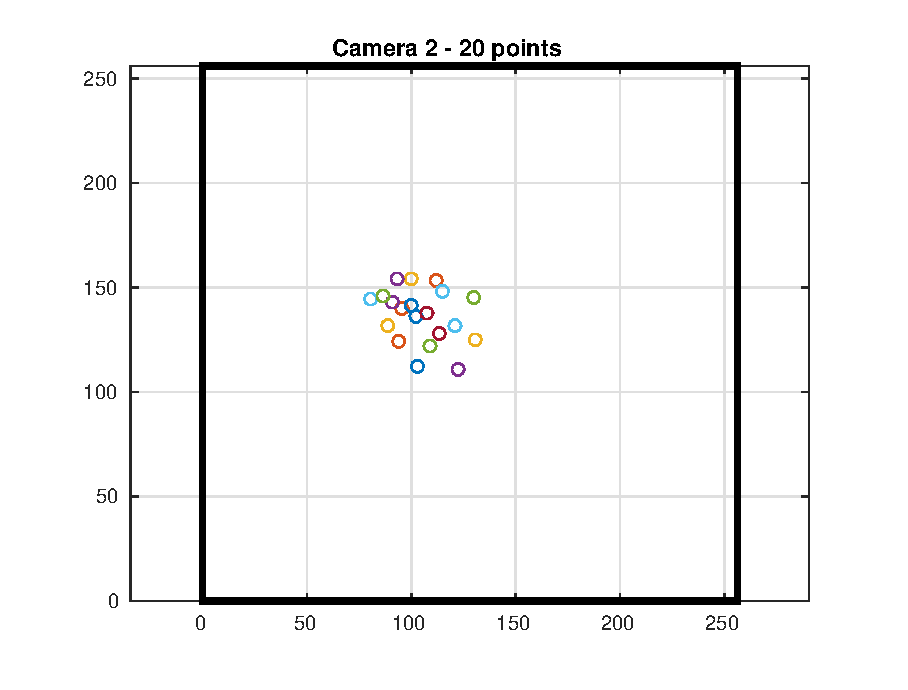
\includegraphics[width=0.4\linewidth]{figures/c2_20.eps}}\\

	\subfigure[50 reference points in camera 1 plane]{\label{c1_50}
		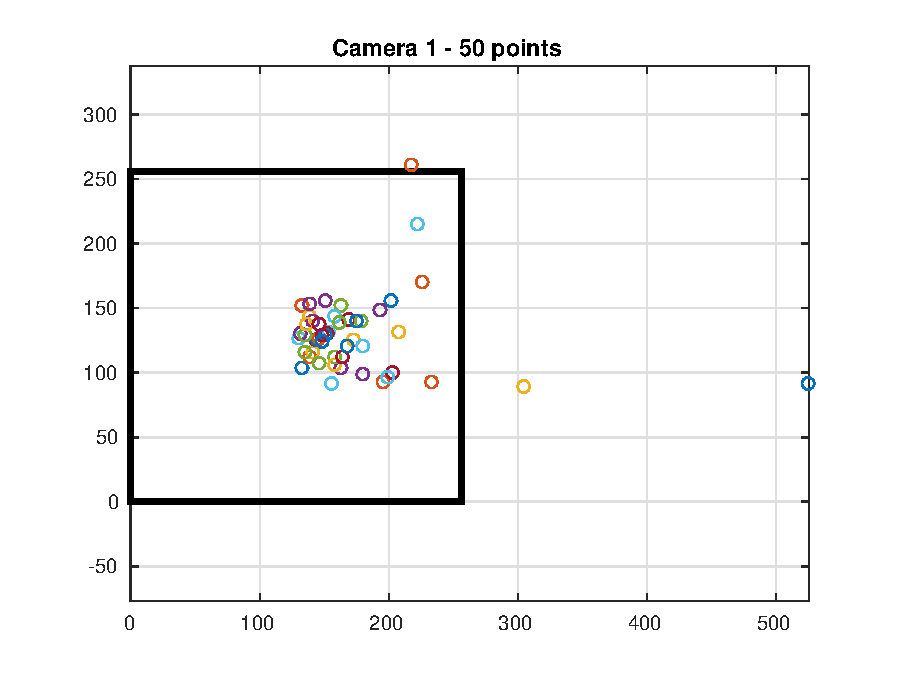
\includegraphics[width=0.4\linewidth]{figures/c1_50.eps}}~
	\subfigure[50 reference points in camera 2 plane]{\label{c2_50}
		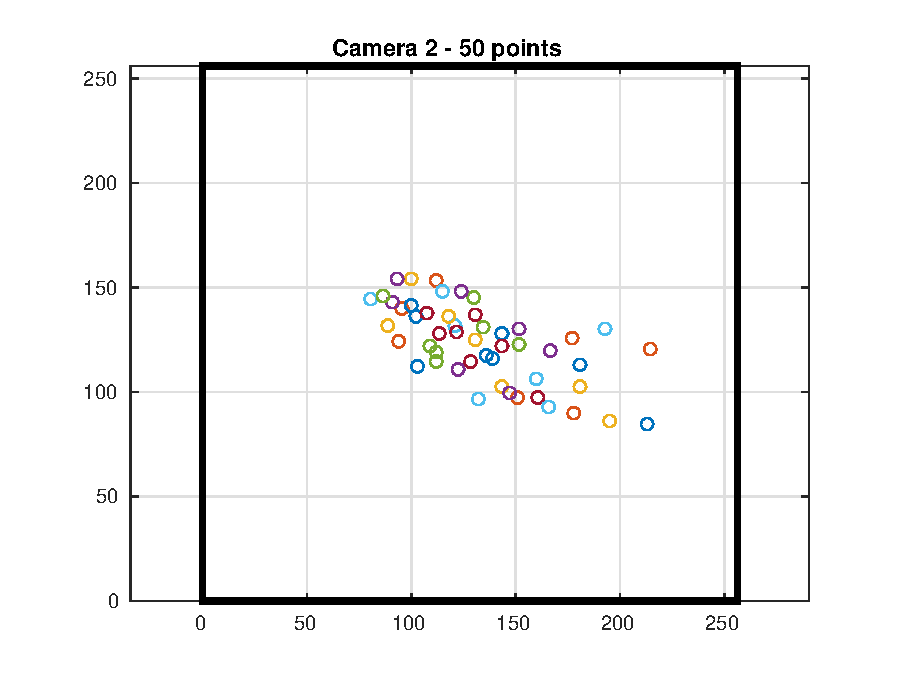
\includegraphics[width=0.4\linewidth]{figures/c2_50.eps}}\\

	\subfigure[150 reference points in camera 1 plane]{\label{c1_150}
		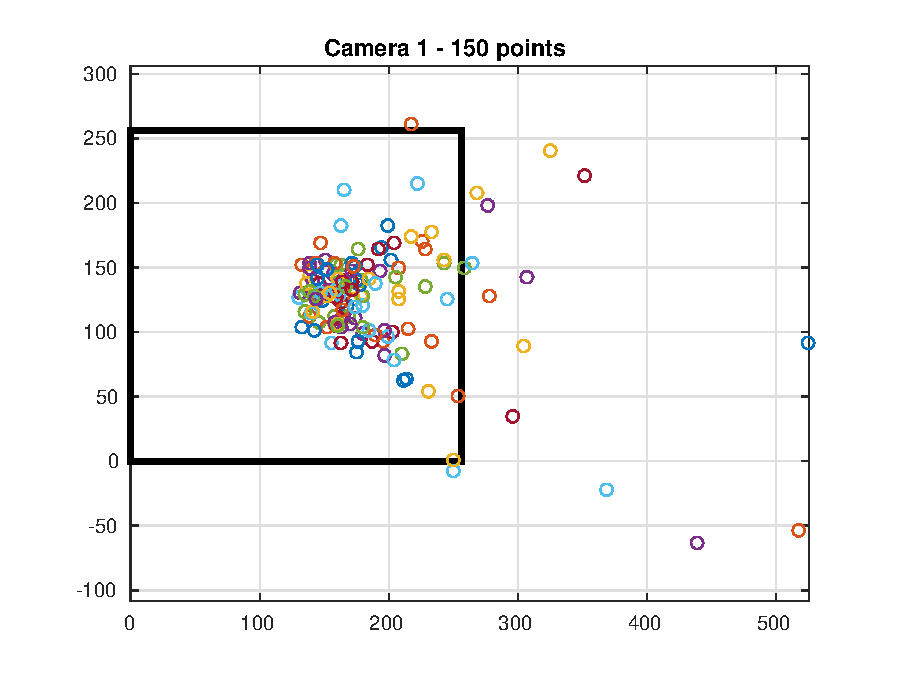
\includegraphics[width=0.4\linewidth]{figures/c1_150.eps}}~
	\subfigure[150 reference points in camera 2 plane]{\label{c2_150}
		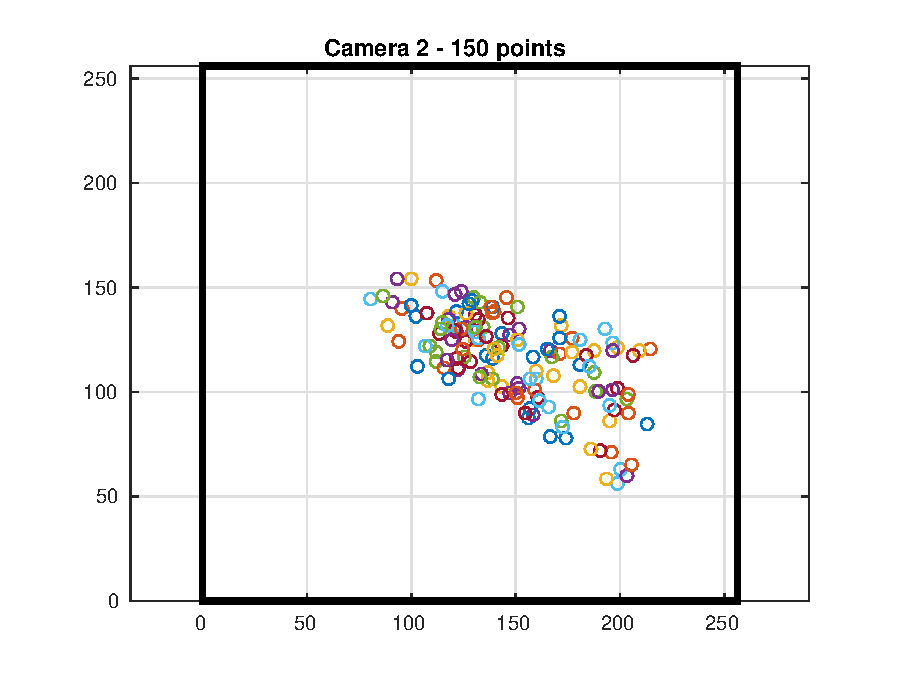
\includegraphics[width=0.4\linewidth]{figures/c2_150.eps}}\\
		
		
	\caption{Sets of 20, 50 and 150 reference points}
	\label{fig:refpoints}
\end{figure}





\subsection{Step 8}

The 8-point method was applied to the set of 20 reference points to calculate the fundamental matrix based only on the projections of the reference points. This was performed by a custom written function \textit{compute\_F}, which computed the fundamental matrix using the 8-point method. This function can be found in Appendix \ref{computeF}.

The code used to perform this operation and the result can be found below.

\begin{verbatim}
% Calculate fundamental matrix using 8-point method
F_8 = compute_F(p1,p2)
\end{verbatim}

\[
F\_8 = 
\begin{bmatrix}
    0.0000  &  0.0001  & -0.0066\\
    0.0000  & -0.0000  &  0.0130\\
   -0.0096  & -0.0173  &  1.0000\\
\end{bmatrix}
\]




\subsection{Step 9}

The objective in this step was to compare the result obtained in the previous step with the ground truth calculated on step 4. For this, we performed an element wise division of the two matrices, to compare each element to their correspondent element. As expected, the result was a matrix filled with ones, which means the elements in both matrices were equal and our estimation was exact. The commands and results are found below.

\begin{verbatim}
% Compare matrices
ratio = F_8./F
\end{verbatim}


\[
ratio = 
\begin{bmatrix}
    1.0000  &  1.0000  &  1.0000\\
    1.0000  &  1.0000  &  1.0000\\
    1.0000  &  1.0000  &  1.0000\\
\end{bmatrix}
\]



\subsection{Step 10}

Our objective in this step was to plot for both cameras all the epipolar lines, projected points and epipoles using the fundamental matrix calculated in step 8. The results can be found in Fig. \ref{fig:epip_clean}. We can see that since no noise has been added to the projections, all the epipolar lines contain their respective projection points and they all cross at the epipoles. The code used for this step can be found below.

\begin{verbatim}
epip1 = normalise_scale(A1*[T;1]);
x = [min(0,epip1(1))-10,max(256,epip1(1))+10];
figure;
% subplot(1,2,1);
hold on;
grid on;
for i = 1:size(p1,2)
    scatter(p1(1,i),p1(2,i),'b');
    lm = F_8'*p2(:,i);
    m = -lm(1)/lm(2);
    d = -lm(3)/lm(2);
    y = m*x + d;
    plot(x,y,'r');
end
plot([0 sx1 sx1 0 0],[0 0 sy1 sy1 0],'k');
scatter(epip1(1),epip1(2),'gh','LineWidth',2);
axis('equal');
title('Camera 1');


epip2 = normalise_scale(A2*[0;0;0;1]);
x = [min(0,epip2(1))-10,max(256,epip2(1))+10];
% subplot(1,2,2);
figure;
hold on;
grid on;
for i = 1:size(p1,2)
    scatter(p2(1,i),p2(2,i),'b');
    lm = F_8*p1(:,i);
    m = -lm(1)/lm(2);
    d = -lm(3)/lm(2);
    y = m*x + d;
    plot(x,y,'r');
end
plot([0 sx2 sx2 0 0],[0 0 sy2 sy2 0],'k');
scatter(epip2(1),epip2(2),'gh','LineWidth',2);
axis('equal');
title('Camera 2');
\end{verbatim}


\begin{figure}[ht]
	\centering

	\subfigure[Epipolar lines in camera 1]{\label{ep_c1_clean}
		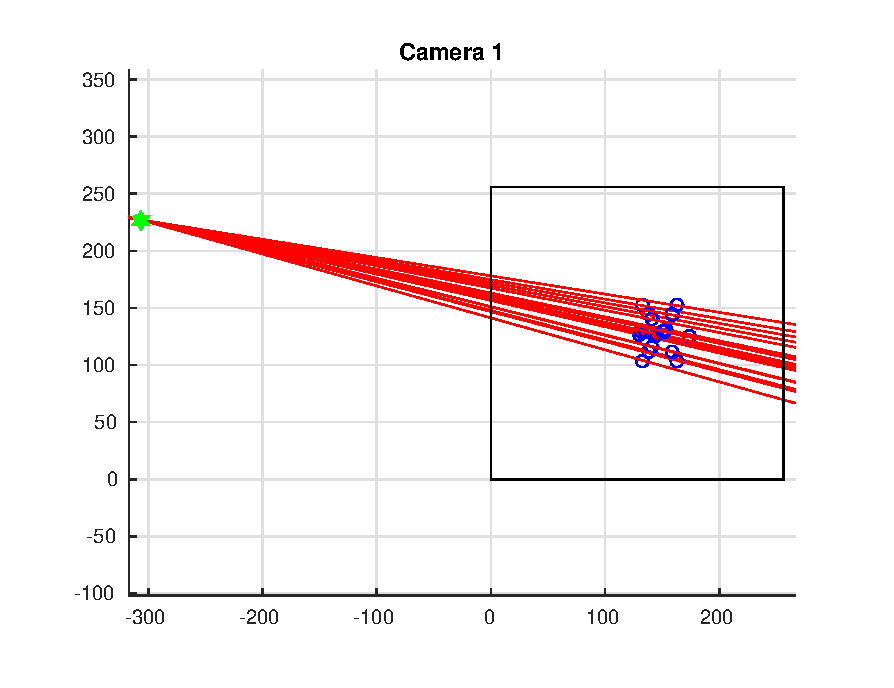
\includegraphics[width=0.4\linewidth]{figures/ep_c1_clean.eps}}~
	\subfigure[Epipolar lines in camera 2]{\label{ep_c2_clean}
		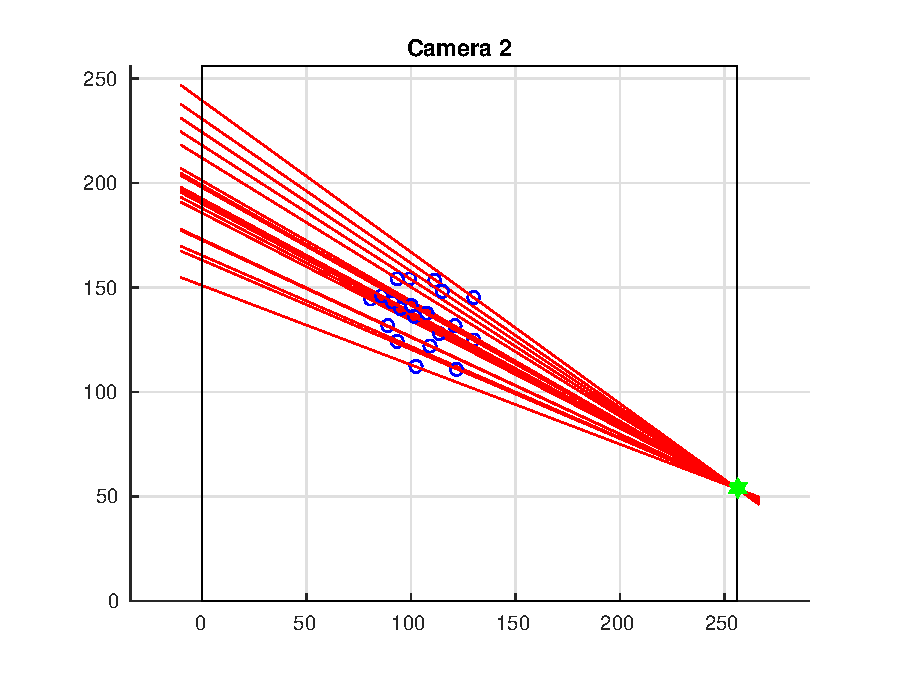
\includegraphics[width=0.4\linewidth]{figures/ep_c2_clean.eps}}\\

	\caption{Epipoles and epipolar lines obtained from the fundamental matrix}
	\label{fig:epip_clean}
\end{figure}



\subsection{Step 11}

In this step, our task was to add Gaussian noise to all projection points (including the sets of 50 and 150 points), with 95\% of the added noise in the range [-1,1]. This was achieved by the following lines of code:

\begin{verbatim}
p1_n = p1 + [0.5*randn(2,size(V,2)); zeros(1,size(V,2))];
p2_n = p2 + [0.5*randn(2,size(V,2)); zeros(1,size(V,2))];

p1_50_n = p1_50 + [0.5*randn(2,size(V50,2)); zeros(1,size(V50,2))];
p2_50_n = p2_50 + [0.5*randn(2,size(V50,2)); zeros(1,size(V50,2))];

p1_150_n = p1_150 + [0.5*randn(2,size(V150,2)); zeros(1,size(V150,2))];
p2_150_n = p2_150 + [0.5*randn(2,size(V150,2)); zeros(1,size(V150,2))];
\end{verbatim}




\subsection{Step 12}

In this step, we calculated again the fundamental matrix using the projection points, only this time we used the projections with added noise calculated in step 11. The results of one example run of this step can be found in Fig. \ref{fig:mse_n1}, where the green marks represent the correct epipoles and the black marks represent the epipole based on the calculated fundamental matrix. 

Table \ref{tab:ep_dist_mse_n1} contains the distance between the correct and estimated epipoles for each case on a given run of the code. We can observe in the table's values that the estimation of the position of the epipoles improves with larger number of points. We also calculated the element wise ratio between the calculated fundamental matrices and the ground truth fundamental matrix. We can see that  larger number of points makes the elements of this ratio go towards one, i.e. the approximation approaches the true fundamental matrix.

In this step an auxiliary function called \textit{plot\_epips} was written, which roughly encompassed steps 8 to 10, since those operations were performed many times. The code of the \textit{plot\_epips} function can be found in Appendix \ref{plotepips}.The code used for this step is displayed below.

\begin{verbatim}
% Calculate everything and compare to true F
[F_mse_20,epip1_diff_F_mse_20,epip2_diff_F_mse_20] = 
    plot_epips(p1_n,p2_n,epip1,epip2,'(20 points, noise [-1,1])')
ratio_mse_20 = F_mse_20./F

[F_mse_50,epip1_diff_F_mse_50,epip2_diff_F_mse_50] =
    plot_epips(p1_50_n,p2_50_n,epip1,epip2,'(50 points, noise [-1,1])')
ratio_mse_50 = F_mse_50./F

[F_mse_150,epip1_diff_F_mse_150,epip2_diff_F_mse_150] =
    plot_epips(p1_150_n,p2_150_n,epip1,epip2,'(150 points, noise [-1,1])')
ratio_mse_150 = F_mse_150./F
\end{verbatim}


\begin{figure}[ht]
	\centering

	\subfigure[Epipolar lines with 20 noisy points in camera 1]{\label{ep_c1_n1_20}
		\includegraphics[width=0.4\linewidth]{figures/ep_c1_n1_20.eps}}~
	\subfigure[Epipolar lines with 20 noisy points in camera 2]{\label{ep_c2_n1_20}
		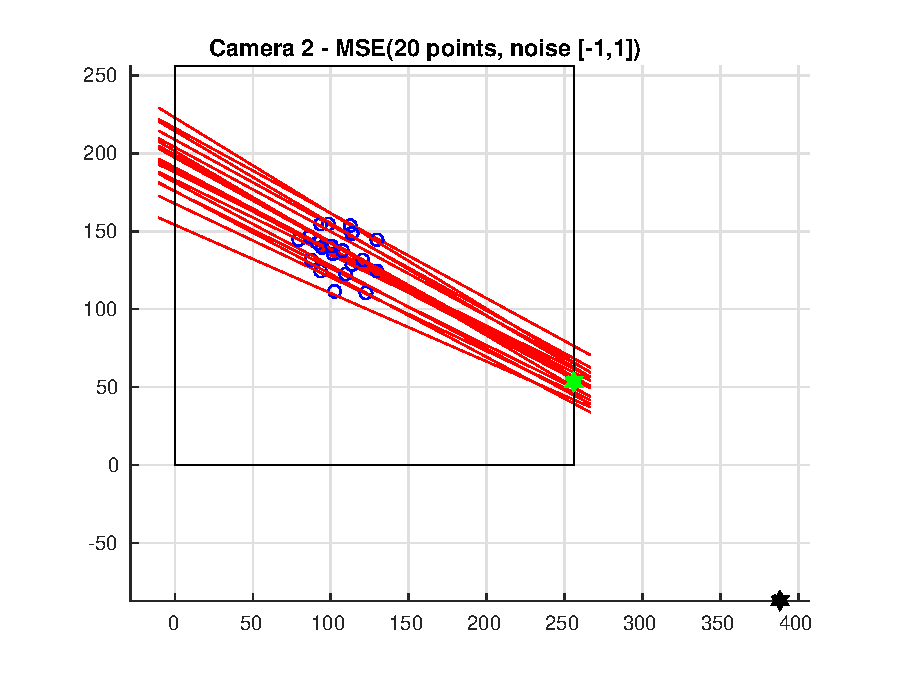
\includegraphics[width=0.4\linewidth]{figures/ep_c2_n1_20.eps}}\\

	\subfigure[Epipolar lines with 50 noisy points in camera 1]{\label{ep_c1_n1_50}
		\includegraphics[width=0.4\linewidth]{figures/ep_c1_n1_50.eps}}~
	\subfigure[Epipolar lines with 50 noisy points in camera 2]{\label{ep_c2_n1_50}
		\includegraphics[width=0.4\linewidth]{figures/ep_c2_n1_50.eps}}\\

	\subfigure[Epipolar lines with 150 noisy points in camera 1]{\label{ep_c1_n1_150}
		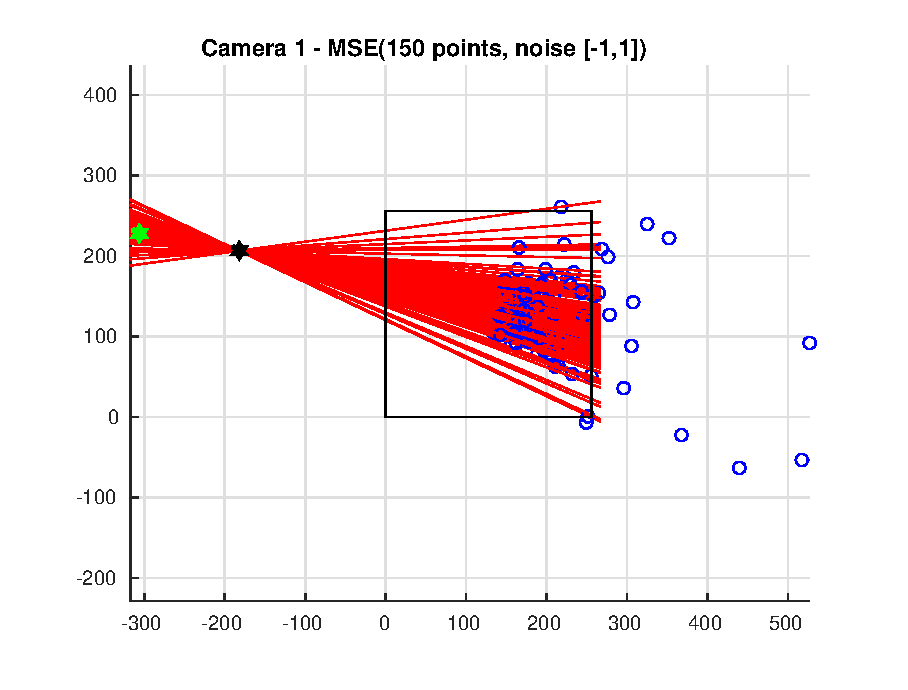
\includegraphics[width=0.4\linewidth]{figures/ep_c1_n1_150.eps}}~
	\subfigure[Epipolar lines with 150 noisy points in camera 2]{\label{ep_c2_n1_150}
		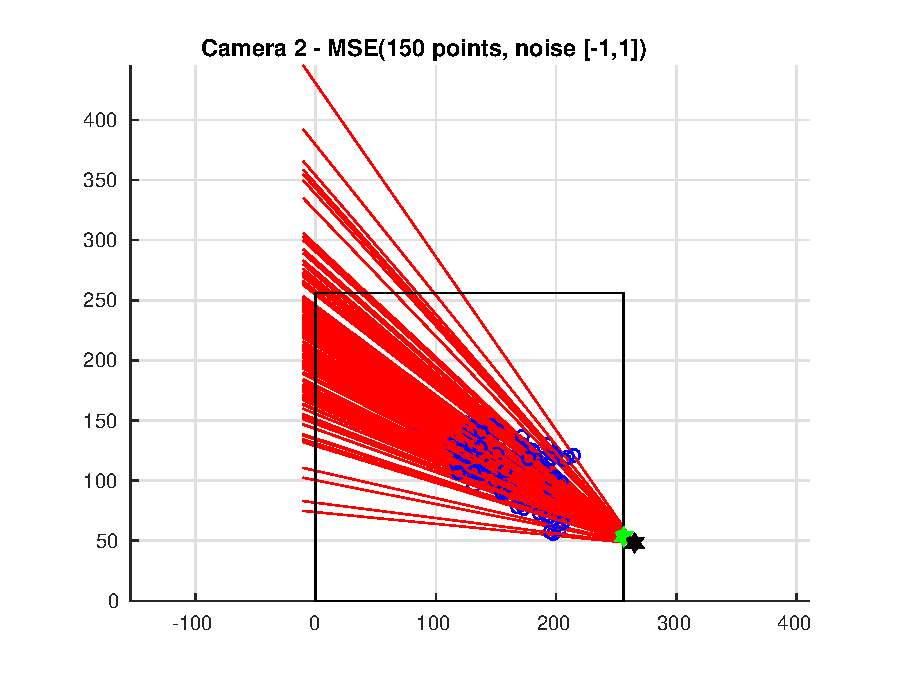
\includegraphics[width=0.4\linewidth]{figures/ep_c2_n1_150.eps}}\\
		
		
	\caption{Epipolar lines using fundamental matrices calculated using MSE with reference points with added Gaussian noise with 95\% in the range [-1,1]}
	\label{fig:mse_n1}
\end{figure}



\[
F\_n1\_mse\_20./F = 
\begin{bmatrix}
    0.6383  & -0.0314  &  0.2704\\
    1.3061  & -0.3899  & -0.3078\\
    0.7185  &  0.1585  &  1.0000\\
\end{bmatrix}
\]


\[
F\_n1\_mse\_50./F = 
\begin{bmatrix}
    0.7082  &  0.1595  &  0.3769\\
    1.3671  &  0.0496  & -0.0479\\
    0.8397  &  0.2863  &  1.0000\\
\end{bmatrix}
\]


\[
F\_n1\_mse\_150./F = 
\begin{bmatrix}
    0.7543  &  0.5725  &  0.6572\\
    1.0007  &  0.2410  &  0.4048\\
    0.8108  &  0.6529  &  1.0000\\
\end{bmatrix}
\]

\begin{table}[ht]
	\caption{Distance between epipoles calculated using MSE with noisy projections (95\% in range [-1,1]) and correct epipoles}
	\centering
	\begin{tabular}{l | r r }\label{tab:ep_dist_mse_n1}
		Number of points & Camera 1 & Camera 2 \\
		\hline
		20 & 415.5559 & 465.3017 \\
		50 & 337.5307 & 181.1066 \\
		150 & 143.0031 & 25.8472 \\
	\end{tabular}
\end{table}


\subsection{Step 13}

In this step, the procedure of steps 11 and 12 were repeated, only this time the 95\% of the added noise was in the range [-2,2]. The results of this step can be found in Fig. \ref{fig:mse_n2}, in Table \ref{tab:ep_dist_mse_n2} and in the ratio matrices below. The code used for this step was the following:

\begin{verbatim}
% Add gaussian noise to projections
p1_n2 = p1 + [randn(2,size(V,2)); zeros(1,size(V,2))];
p2_n2 = p2 + [randn(2,size(V,2)); zeros(1,size(V,2))];

p1_50_n2 = p1_50 + [randn(2,size(V50,2)); zeros(1,size(V50,2))];
p2_50_n2 = p2_50 + [randn(2,size(V50,2)); zeros(1,size(V50,2))];

p1_150_n2 = p1_150 + [randn(2,size(V150,2)); zeros(1,size(V150,2))];
p2_150_n2 = p2_150 + [randn(2,size(V150,2)); zeros(1,size(V150,2))];


% Calculate everything and compare to true F
[F_mse2_20,epip1_diff_F_mse2_20,epip2_diff_F_mse2_20] =
    plot_epips(p1_n2,p2_n2,epip1,epip2,'(20 points, noise [-2,2])')
ratio_mse2_20 = F_mse2_20./F

[F_mse2_50,epip1_diff_F_mse2_50,epip2_diff_F_mse2_50] =
    plot_epips(p1_50_n2,p2_50_n2,epip1,epip2,'(50 points, noise [-2,2])')
ratio_mse2_50 = F_mse2_50./F

[F_mse2_150,epip1_diff_F_mse2_150,epip2_diff_F_mse2_150] =
    plot_epips(p1_150_n2,p2_150_n2,epip1,epip2,'(150 points, noise [-2,2])')
ratio_mse2_150 = F_mse2_150./F
\end{verbatim}

\begin{figure}[ht]
	\centering

	\subfigure[Epipolar lines with 20 noisy points in camera 1]{\label{ep_c1_n2_20}
		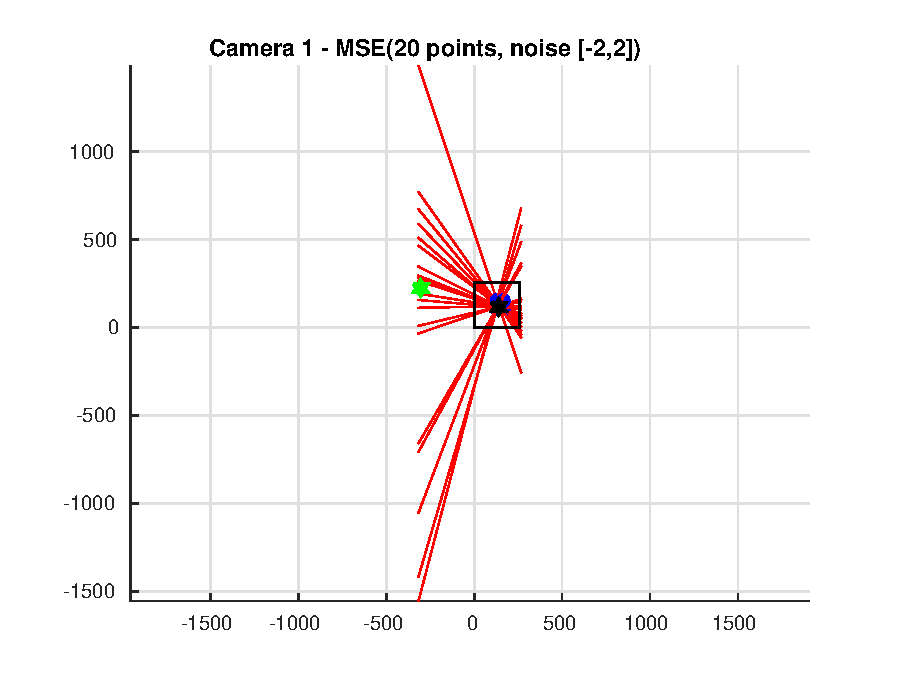
\includegraphics[width=0.4\linewidth]{figures/ep_c1_n2_20.eps}}~
	\subfigure[Epipolar lines with 20 noisy points in camera 2]{\label{ep_c2_n2_20}
		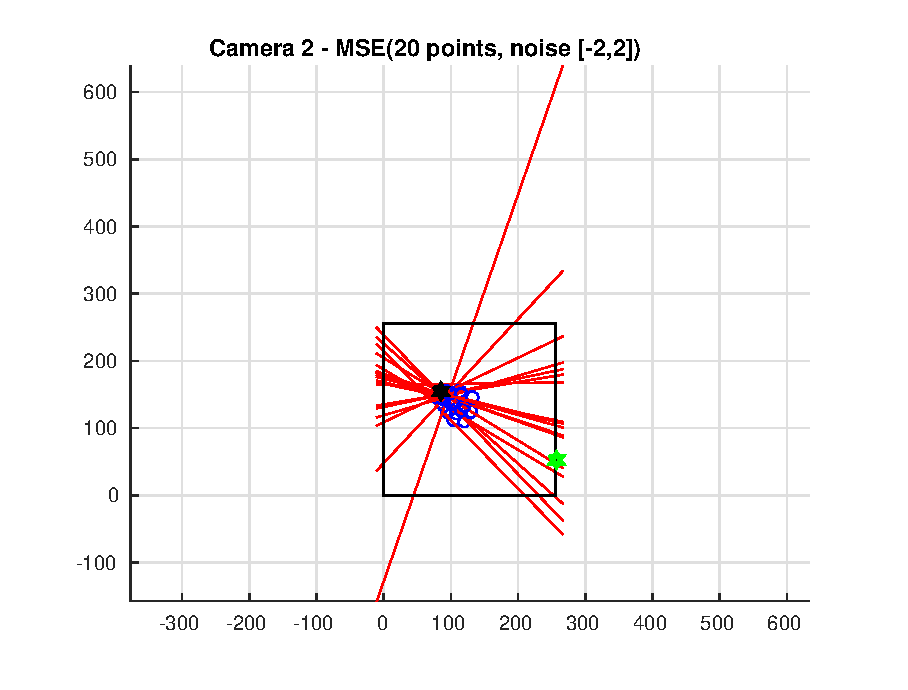
\includegraphics[width=0.4\linewidth]{figures/ep_c2_n2_20.eps}}\\

	\subfigure[Epipolar lines with 50 noisy points in camera 1]{\label{ep_c1_n2_50}
		\includegraphics[width=0.4\linewidth]{figures/ep_c1_n2_50.eps}}~
	\subfigure[Epipolar lines with 50 noisy points in camera 2]{\label{ep_c2_n2_50}
		\includegraphics[width=0.4\linewidth]{figures/ep_c2_n2_50.eps}}\\

	\subfigure[Epipolar lines with 150 noisy points in camera 1]{\label{ep_c1_n2_150}
		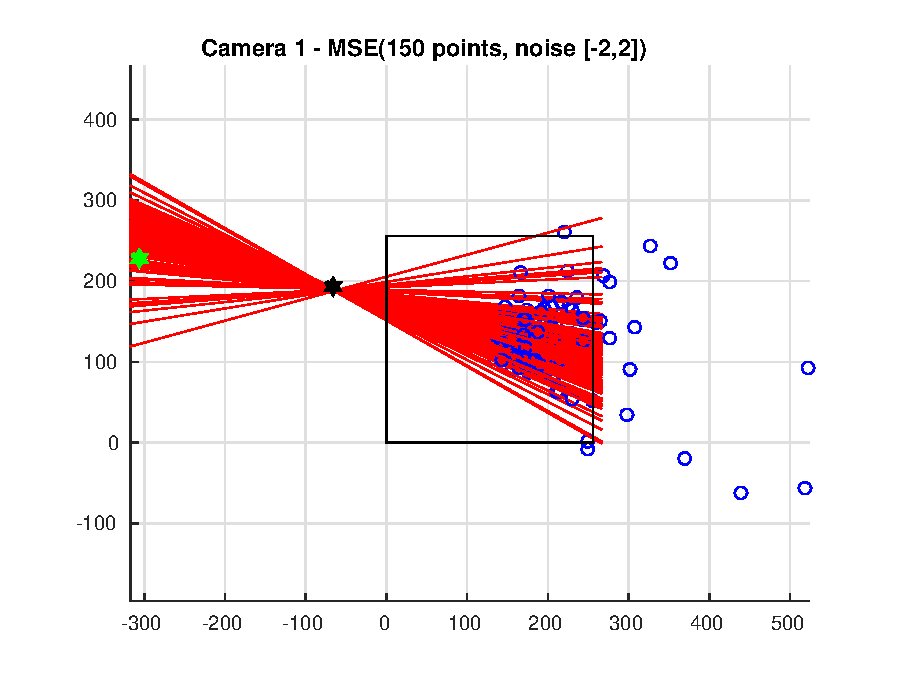
\includegraphics[width=0.4\linewidth]{figures/ep_c1_n2_150.eps}}~
	\subfigure[Epipolar lines with 150 noisy points in camera 2]{\label{ep_c2_n2_150}
		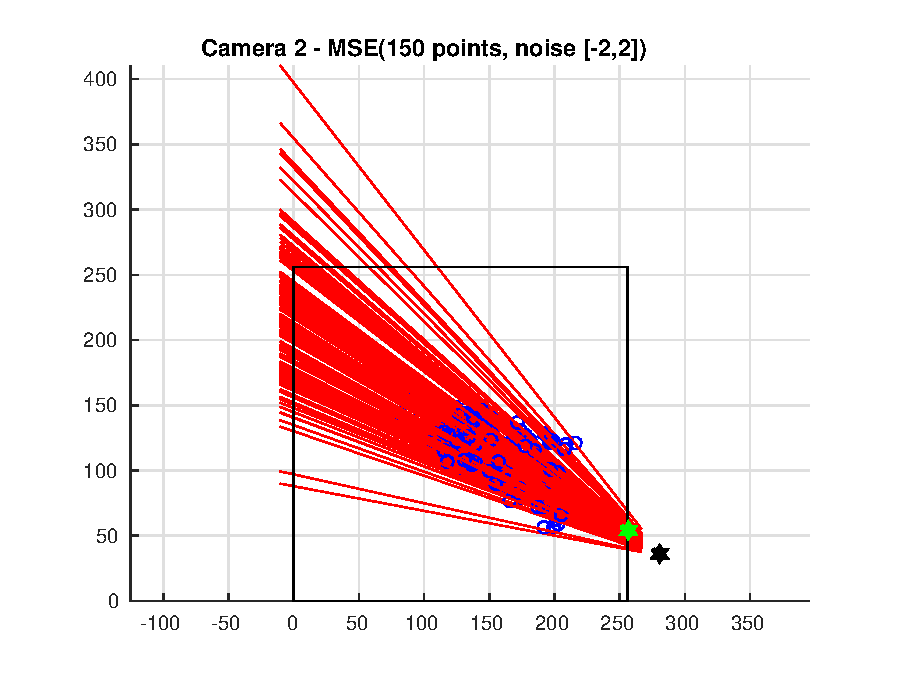
\includegraphics[width=0.4\linewidth]{figures/ep_c2_n2_150.eps}}\\
		
		
	\caption{Epipolar lines using fundamental matrices calculated using MSE with reference points with added Gaussian noise with 95\% in the range [-2,2]}
	\label{fig:mse_n2}
\end{figure}


\[
F\_n2\_mse\_20./F = 
\begin{bmatrix}
    0.7061  & -0.1798  &  0.3239\\
    1.1293  & -0.6395  & -0.4978\\
    0.6216  &  0.0097  &  1.0000\\
\end{bmatrix}
\]


\[
F\_n2\_mse\_50./F = 
\begin{bmatrix}
    0.5729  &  0.0163  &  0.2447\\
    1.2392  & -0.4344  & -0.2785\\
    0.7066  &  0.1978  &  1.0000\\
\end{bmatrix}
\]


\[
F\_n2\_mse\_150./F = 
\begin{bmatrix}
    0.5601  &  0.2325  &  0.4113\\
    0.9786  & -0.2976  & -0.0682\\
    0.6503  &  0.3584  &  1.0000\\
\end{bmatrix}
\]

\begin{table}[ht]
	\caption{Distance between epipoles calculated using MSE with noisy projections (95\% in range [-2,2]) and correct epipoles}
	\centering
	\begin{tabular}{l | r r }\label{tab:ep_dist_mse_n2}
		Number of points & Camera 1 & Camera 2 \\
		\hline
		20 & 482.5575 & 147.7943 \\
		50 & 387.6754 & 658.1037 \\
		150 & 295.8707 & 140.3587 \\
	\end{tabular}
\end{table}


%%%%%%%%%%%%%%%%%%%%%%%%%%%%%%%%%%%%%%%%%%%%%%%%%%%%%%%%%%%%%%%%%%%%%%%%%%%%%%%
\newpage
\section{Part 2}\label{p2}

\subsection{Step 14}

On this step, a function to calculate the fundamental matrix given a set of pairs of projections using SVD was implemented. This function, called \textit{compute\_F\_svd}, can be found in Appendix \ref{fsvd}. We then applied this function to calculate the fundamental matrix using the set of 20 projections with no added noise and compared the results with the ground truth fundamental matrix. As expected, the result was very precise once again. The code and results for this step can be found below.

\begin{verbatim}
% Calculate the fundamental matrix using SVD
F_8_svd = compute_F_svd(p1,p2);
ratio_svd = F_8_svd./F_8
\end{verbatim}

\[
ratio\_svd = 
\begin{bmatrix}
    1.0000  &  1.0000  &  1.0000\\
    1.0000  &  1.0000  &  1.0000\\
    1.0000  &  1.0000  &  1.0000\\
\end{bmatrix}
\]



\subsection{Step 15}

On this step, the procedures of steps 11 to 13 were repeated, but using the SVD method to calculate the fundamental matrices using the noisy projections. Once again, an auxiliary function called \textit{plot\_epips\_svd} was written since the same process was repeatedly applied on different sets of points. This function can be found in Appendix \ref{almostover}.

The results of this steps can be found in Figures \ref{fig:svd_n1} and \ref{fig:svd_n2}, and also in Tables \ref{tab:ep_dist_svd_n1} and \ref{tab:ep_dist_svd_n2}, as well as in the ratio matrices below. Once again, we see that generally a larger number of points leads to a more precise approximation of the fundamental matrix, but in this specific run we observe that the noise added to the set of 50 projections led to an unexpected behaviour and to a worse approximation of the ground truth fundamental matrix. Once again, the approximation using 150 points achieved the best precision among the simulated scenarios.

The code used for the computations in this step are displayed below.

\begin{verbatim}
% Calculate everything and compare to true F
[F_svd_20,epip1_diff_F_svd_20,epip2_diff_F_svd_20] =
    plot_epips_svd(p1_n,p2_n,epip1,epip2,'(20 points, noise [-1,1])')
ratio_svd_20 = F_svd_20./F

[F_svd_50,epip1_diff_F_svd_50,epip2_diff_F_svd_50] =
    plot_epips_svd(p1_50_n,p2_50_n,epip1,epip2,'(50 points, noise [-1,1])')
ratio_svd_50 = F_svd_50./F

[F_svd_150,epip1_diff_F_svd_150,epip2_diff_F_svd_150] =
    plot_epips_svd(p1_150_n,p2_150_n,epip1,epip2,'(150 points, noise [-1,1])')
ratio_svd_150 = F_svd_150./F


%% Step 15-2

% Calculate everything and compare to true F
[F_svd2_20,epip1_diff_F_svd2_20,epip2_diff_F_svd2_20] =
    plot_epips_svd(p1_n2,p2_n2,epip1,epip2,'(20 points, noise [-2,2])')
ratio_svd2_20 = F_svd2_20./F

[F_svd2_50,epip1_diff_F_svd2_50,epip2_diff_F_svd2_50] =
    plot_epips_svd(p1_50_n2,p2_50_n2,epip1,epip2,'(50 points, noise [-2,2])')
ratio_svd2_50 = F_svd2_50./F

[F_svd2_150,epip1_diff_F_svd2_150,epip2_diff_F_svd2_150] =
  plot_epips_svd(p1_150_n2,p2_150_n2,epip1,epip2,'(150 points, noise [-2,2])')
ratio_svd2_150 = F_svd2_150./F
\end{verbatim}


\begin{figure}[ht]
	\centering

	\subfigure[Epipolar lines with 20 noisy points in camera 1]{\label{ep_c1_n1_20_svd}
		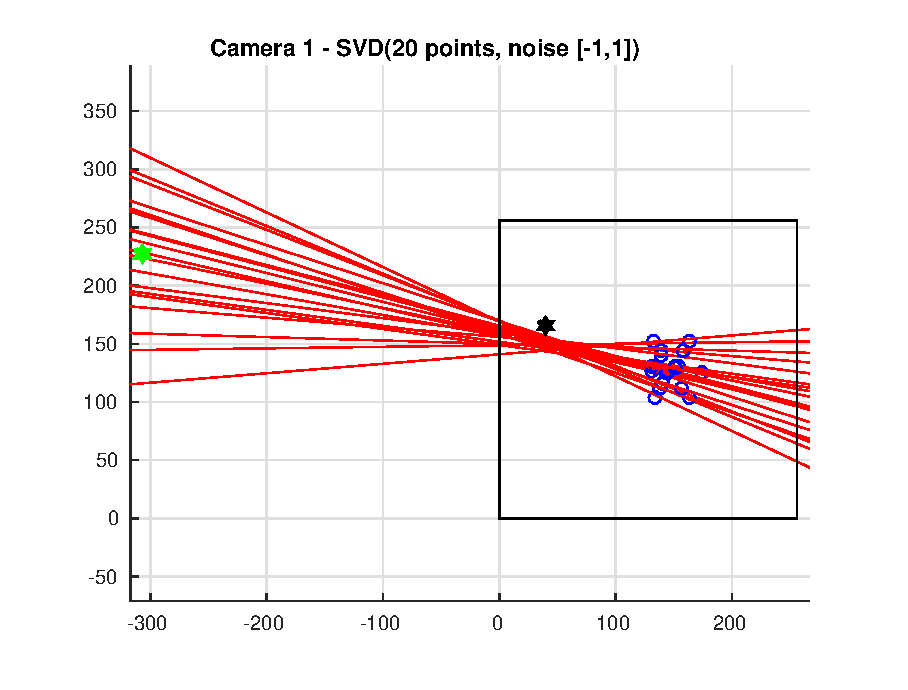
\includegraphics[width=0.4\linewidth]{figures/ep_c1_n1_20_svd.eps}}~
	\subfigure[Epipolar lines with 20 noisy points in camera 2]{\label{ep_c2_n1_20_svd}
		\includegraphics[width=0.4\linewidth]{figures/ep_c2_n1_20_svd.eps}}\\

	\subfigure[Epipolar lines with 50 noisy points in camera 1]{\label{ep_c1_n1_50_svd}
		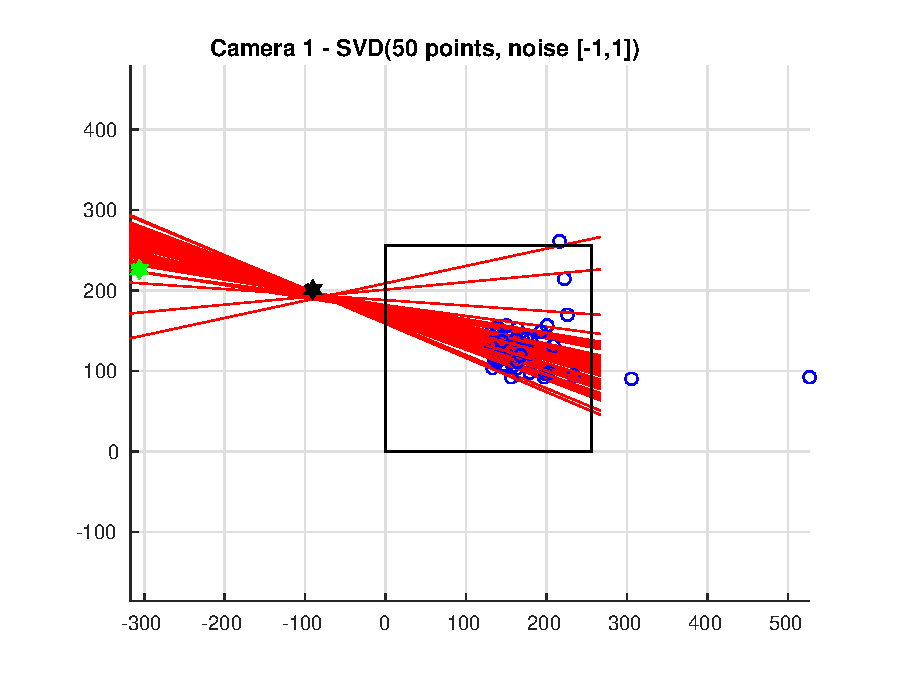
\includegraphics[width=0.4\linewidth]{figures/ep_c1_n1_50_svd.eps}}~
	\subfigure[Epipolar lines with 50 noisy points in camera 2]{\label{ep_c2_n1_50_svd}
		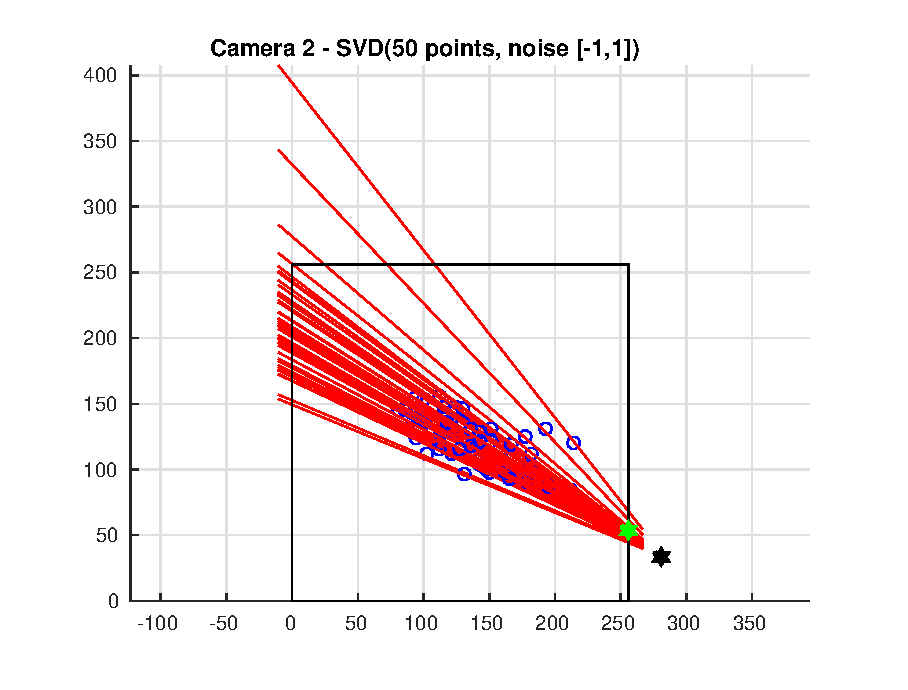
\includegraphics[width=0.4\linewidth]{figures/ep_c2_n1_50_svd.eps}}\\

	\subfigure[Epipolar lines with 150 noisy points in camera 1]{\label{ep_c1_n1_150_svd}
		\includegraphics[width=0.4\linewidth]{figures/ep_c1_n1_150_svd.eps}}~
	\subfigure[Epipolar lines with 150 noisy points in camera 2]{\label{ep_c2_n1_150_svd}
		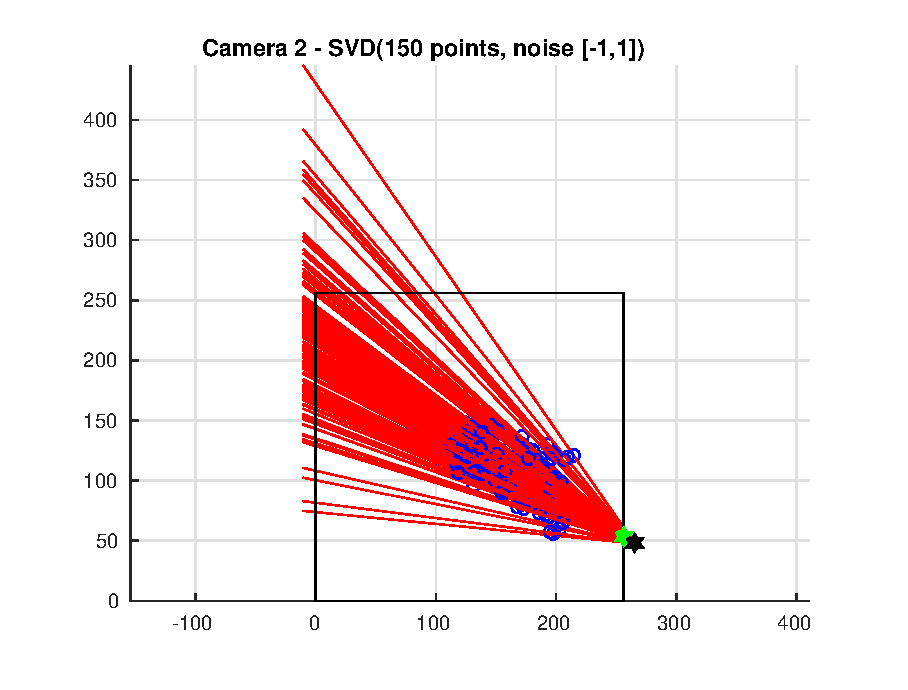
\includegraphics[width=0.4\linewidth]{figures/ep_c2_n1_150_svd.eps}}\\
		
		
	\caption{Epipolar lines using fundamental matrices calculated using SVD with reference points with added Gaussian noise with 95\% in the range [-1,1]}
	\label{fig:svd_n1}
\end{figure}

\[
F\_svd1\_20./F = 
\begin{bmatrix}
    0.6383  & -0.0314  &  0.2704\\
    1.3062  & -0.3899  & -0.3078\\
    0.7185  &  0.1585  &  1.0000\\
\end{bmatrix}
\]


\[
F\_svd1\_50./F = 
\begin{bmatrix}
    0.7082  &  0.1595  &  0.3769\\
    1.3671  &  0.0497  & -0.0479\\
    0.8398  &  0.2863  &  1.0000\\
\end{bmatrix}
\]


\[
F\_svd1\_150./F = 
\begin{bmatrix}
    0.7544  &  0.5726  &  0.6573\\
    1.0006  &  0.2412  &  0.4050\\
    0.8108  &  0.6530  &  1.0000\\
\end{bmatrix}
\]

\begin{table}[ht]
	\caption{Distance between epipoles calculated using SVD with noisy projections (95\% in range [-1,1]) and correct epipoles}
	\centering
	\begin{tabular}{l | r r }\label{tab:ep_dist_svd_n1}
		Number of points & Camera 1 & Camera 2 \\
		\hline
		20 & 415.5530 & 465.3178 \\
		50 & 337.5196 & 181.0491 \\
		150 & 142.9586 & 25.8348 \\
	\end{tabular}
\end{table}



\begin{figure}[ht]
	\centering

	\subfigure[Epipolar lines with 20 noisy points in camera 1]{\label{ep_c1_n2_20_svd}
		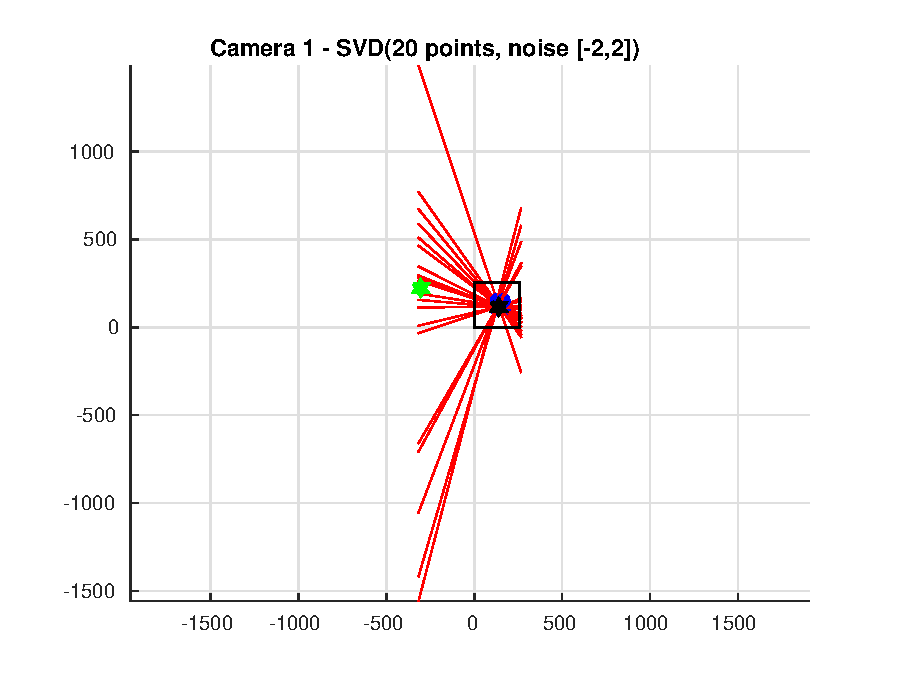
\includegraphics[width=0.4\linewidth]{figures/ep_c1_n2_20_svd.eps}}~
	\subfigure[Epipolar lines with 20 noisy points in camera 2]{\label{ep_c2_n2_20_svd}
		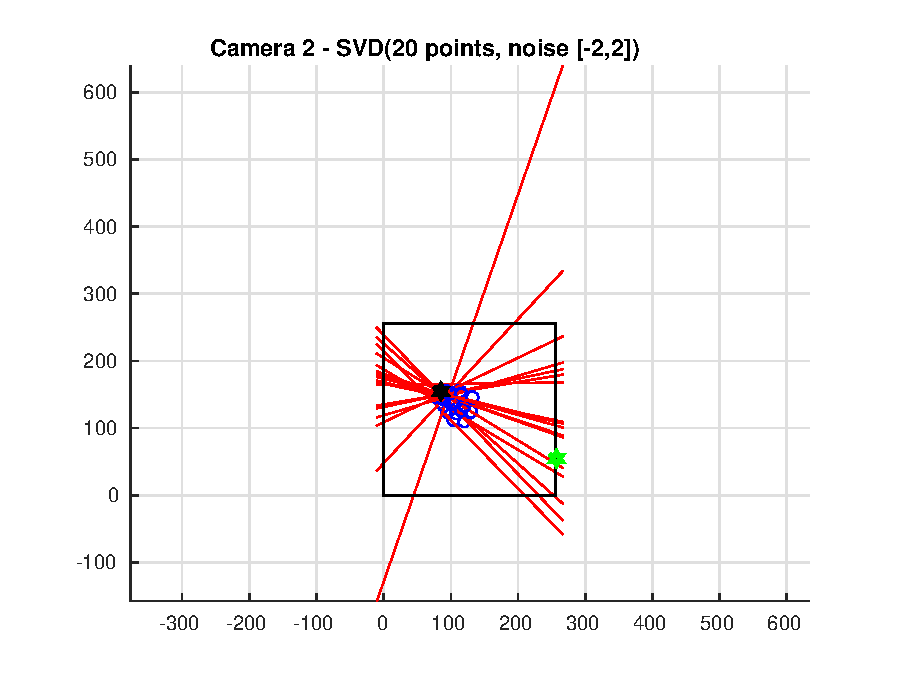
\includegraphics[width=0.4\linewidth]{figures/ep_c2_n2_20_svd.eps}}\\

	\subfigure[Epipolar lines with 50 noisy points in camera 1]{\label{ep_c1_n2_50_svd}
		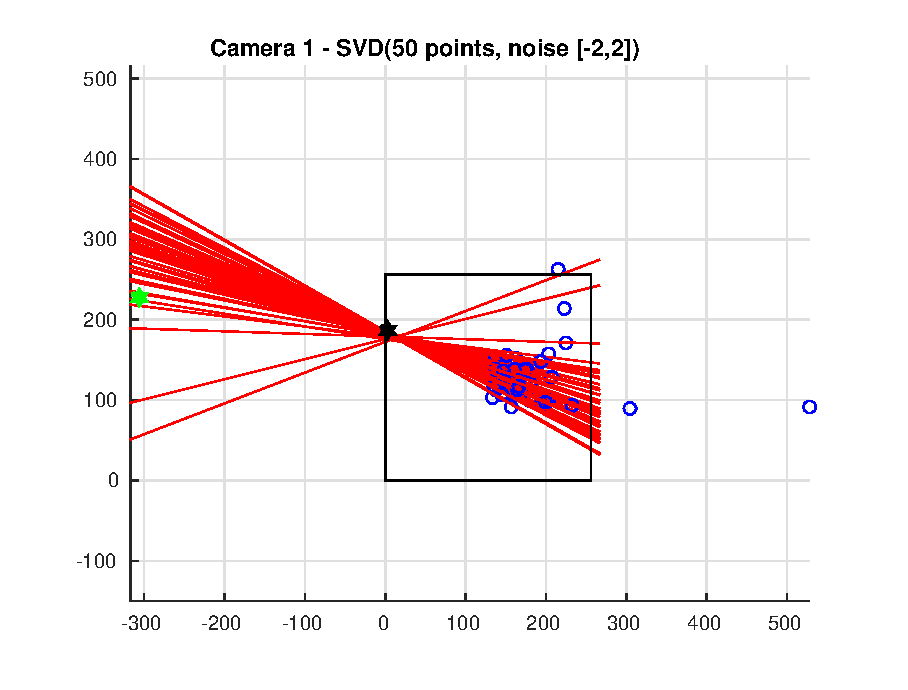
\includegraphics[width=0.4\linewidth]{figures/ep_c1_n2_50_svd.eps}}~
	\subfigure[Epipolar lines with 50 noisy points in camera 2]{\label{ep_c2_n2_50_svd}
		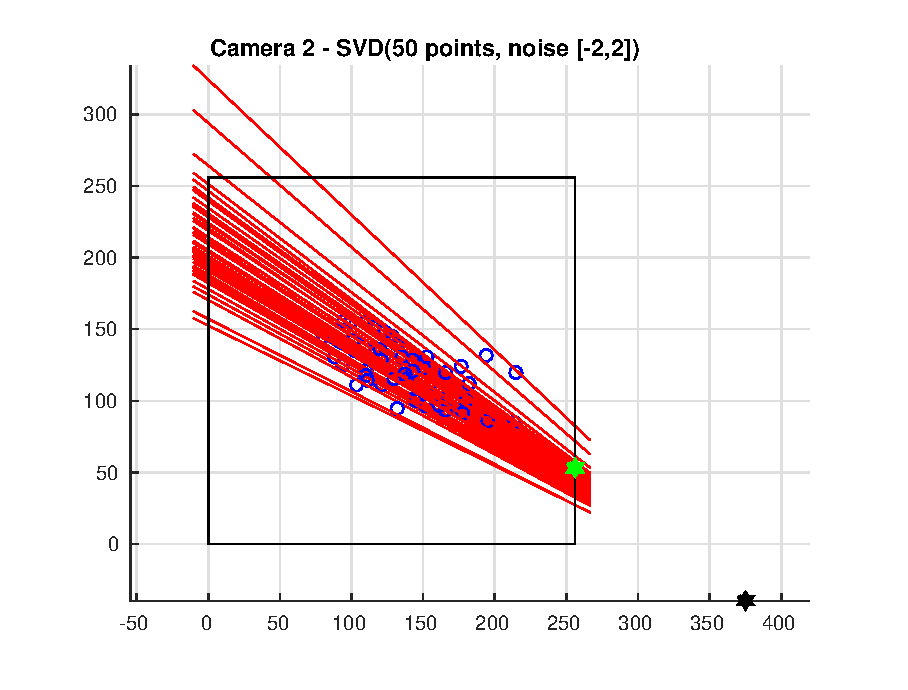
\includegraphics[width=0.4\linewidth]{figures/ep_c2_n2_50_svd.eps}}\\

	\subfigure[Epipolar lines with 150 noisy points in camera 1]{\label{ep_c1_n2_150_svd}
		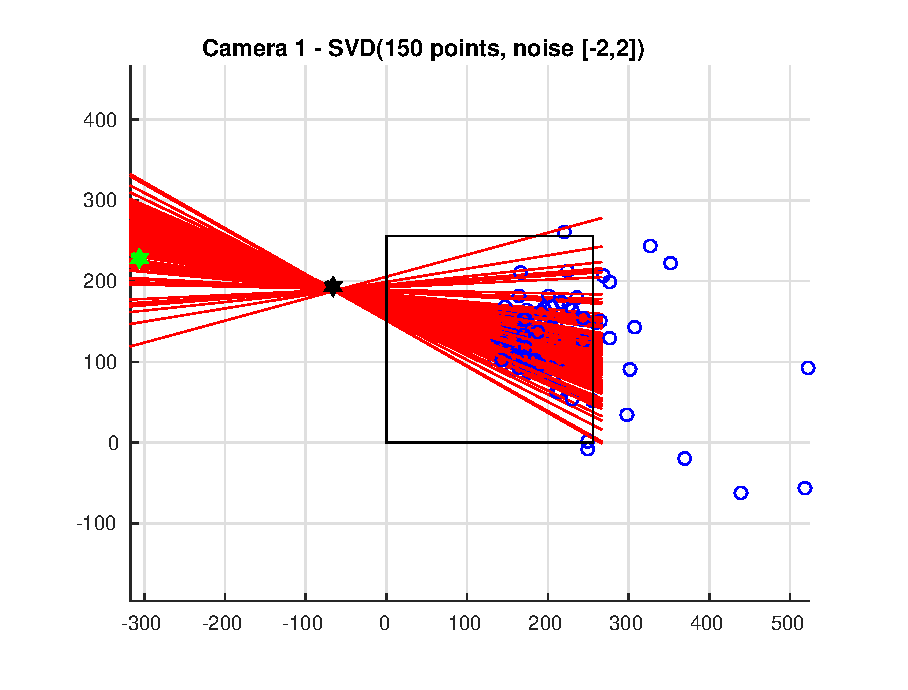
\includegraphics[width=0.4\linewidth]{figures/ep_c1_n2_150_svd.eps}}~
	\subfigure[Epipolar lines with 150 noisy points in camera 2]{\label{ep_c2_n2_150_svd}
		\includegraphics[width=0.4\linewidth]{figures/ep_c2_n2_150_svd.eps}}\\
		
	\caption{Epipolar lines using fundamental matrices calculated using SVD with reference points with added Gaussian noise with 95\% in the range [-2,2]}
	\label{fig:svd_n2}
\end{figure}


\[
F\_svd2\_20./F = 
\begin{bmatrix}
    0.7061  & -0.1799  &  0.3238\\
    1.1293  & -0.6395  & -0.4978\\
    0.6216  &  0.0097  &  1.0000\\
\end{bmatrix}
\]


\[
F\_svd2\_50./F = 
\begin{bmatrix}
    0.5729  &  0.0163  &  0.2447\\
    1.2392  & -0.4344  & -0.2785\\
    0.7066  &  0.1978  &  1.0000\\
\end{bmatrix}
\]


\[
F\_svd2\_150./F = 
\begin{bmatrix}
    0.5601  &  0.2325  &  0.4113\\
    0.9785  & -0.2975  & -0.0681\\
    0.6503  &  0.3584  &  1.0000\\
\end{bmatrix}
\]

\begin{table}[H]
	\caption{Distance between epipoles calculated using SVD with noisy projections (95\% in range [-2,2]) and correct epipoles}
	\centering
	\begin{tabular}{l | r r }\label{tab:ep_dist_svd_n2}
		Number of points & Camera 1 & Camera 2 \\
		\hline
		20 & 482.5572 & 147.7938 \\
		50 & 387.6756 & 658.1093 \\
		150 & 295.8559 & 140.3172 \\
	\end{tabular}
\end{table}


\subsection{Step 16}

In this step we compared the precision of the MSE and SVD methods of estimating the fundamental matrix. We calculated the average distance between each point and their respective epipolar line for all the cases that were simulated with 95\% of the added noise in the range [-1,1]. The results of these calculations can be seen in Table \ref{tab:ep_dist_comp}. We can see that the performance of the MSE and SVD methods are almost equal, but the SVD method is marginally better in every case. We can also clearly see in this table that using more points for estimating the fundamental matrix leads to a more precise result.

The code used for this step is displayed below.

\begin{verbatim}
% 20 points
dist_ls = 0;
dist_svd = 0;
for i = 1:size(p1,2)
    % Least squares total distance
    lm = F_mse_20'*p2_n(:,i);
    dist_ls = dist_ls + abs(lm(1)*p1_n(1,i) + 
        lm(2)*p1_n(2,i) + lm(3))/norm(lm(1:2));
    lm = F_mse_20*p1_n(:,i);
    dist_ls = dist_ls + abs(lm(1)*p2_n(1,i) + 
        lm(2)*p2_n(2,i) + lm(3))/norm(lm(1:2));
    
    % SVD total distance
    lm = F_svd_20'*p2_n(:,i);
    dist_svd = dist_svd + abs(lm(1)*p1_n(1,i) + 
        lm(2)*p1_n(2,i) + lm(3))/norm(lm(1:2));
    lm = F_svd_20*p1_n(:,i);
    dist_svd = dist_svd + abs(lm(1)*p2_n(1,i) + 
        lm(2)*p2_n(2,i) + lm(3))/norm(lm(1:2));
end
mean_dist_ls_20 = dist_ls / (2 * size(p1,2))
mean_dist_svd_20 = dist_svd / (2 * size(p1,2))


% 50 points
dist_ls = 0;
dist_svd = 0;
for i = 1:size(p1_50,2)
    % Least squares total distance
    lm = F_mse_50'*p2_50_n(:,i);
    dist_ls = dist_ls + abs(lm(1)*p1_50_n(1,i) + 
        lm(2)*p1_50_n(2,i) + lm(3))/norm(lm(1:2));
    lm = F_mse_50*p1_50_n(:,i);
    dist_ls = dist_ls + abs(lm(1)*p2_50_n(1,i) + 
        lm(2)*p2_50_n(2,i) + lm(3))/norm(lm(1:2));
    
    % SVD total distance
    lm = F_svd_50'*p2_50_n(:,i);
    dist_svd = dist_svd + abs(lm(1)*p1_50_n(1,i) + 
        lm(2)*p1_50_n(2,i) + lm(3))/norm(lm(1:2));
    lm = F_svd_50*p1_50_n(:,i);
    dist_svd = dist_svd + abs(lm(1)*p2_50_n(1,i) + 
        lm(2)*p2_50_n(2,i) + lm(3))/norm(lm(1:2));
end
mean_dist_ls_50 = dist_ls / (2 * size(p1_50,2))
mean_dist_svd_50 = dist_svd / (2 * size(p1_50,2))


% 150 points
dist_ls = 0;
dist_svd = 0;
for i = 1:size(p1_150,2)
    % Least squares total distance
    lm = F_mse_150'*p2_150_n(:,i);
    dist_ls = dist_ls + abs(lm(1)*p1_150_n(1,i) + 
        lm(2)*p1_150_n(2,i) + lm(3))/norm(lm(1:2));
    lm = F_mse_150*p1_150_n(:,i);
    dist_ls = dist_ls + abs(lm(1)*p2_150_n(1,i) + 
        lm(2)*p2_150_n(2,i) + lm(3))/norm(lm(1:2));
    
    % SVD total distance
    lm = F_svd_150'*p2_150_n(:,i);
    dist_svd = dist_svd + abs(lm(1)*p1_150_n(1,i) + 
        lm(2)*p1_150_n(2,i) + lm(3))/norm(lm(1:2));
    lm = F_svd_150*p1_150_n(:,i);
    dist_svd = dist_svd + abs(lm(1)*p2_150_n(1,i) + 
        lm(2)*p2_150_n(2,i) + lm(3))/norm(lm(1:2));
end
mean_dist_ls_150 = dist_ls / (2 * size(p1_150,2))
mean_dist_svd_150 = dist_svd / (2 * size(p1_150,2))
\end{verbatim}



\begin{table}[ht]
	\caption{Mean distance between points and their correspondent epipolar lines for each simulated case}
	\centering
	\begin{tabular}{l | r r }\label{tab:ep_dist_comp}
		Number of points & MSE & SVD \\
		\hline
		20 & 1.6187 & 1.6186 \\
		50 & 1.0701 & 1.0700 \\
		150 & 0.7574 & 0.7573 \\
	\end{tabular}
\end{table}










%%%%%%%%%%%%%%%%%%%%%%%%%%%%%%%%%%%%%%%%%%%%%%%%%%%%%%%%%%%%%%%%%%%%%%%%%%%%%%%
\section{Conclusion}\label{conclusion}

We demonstrated two different ways of calculating the fundamental matrix using only a set of projections with the 8-point method, one using MSE and one using SVD. We concluded that the SVD method is marginally more precise, but the performance of both methods is very similar.

We also observed that the addition of noise highly influences the obtained results. Even using 20 points and added noise in the order of 1 pixel the results were very bad, but using a larger number of points, such as 150, resulted on a more stable estimation of the fundamental matrix.






%%%%%%%%%%%%%%%%%%%%%%%%%%%%%%%%%%%%%%%%%%%%%%%%%%%%%%%%%%%%%%%%%%%%%%%%%%%%%%%
\appendices

%%%%%%%%%%%%%%%%%%%%%%%%%%%%%%%%%%%%%%%%%%%%%%%%%%%%%%%%%%%%%%%%%%%%%%%%%%%%%%%
\newpage
\section{compute\_F.m}\label{computeF}

\begin{verbatim}
function F = compute_F(p1,p2)
% Compute fundamental matrix based on projections on 2 different cameras

assert(size(p1,2) == size(p2,2))
assert(size(p1,2) > 7)
assert(size(p1,1) == size(p2,1))
assert(size(p1,1) == 3)

p1_n = normalise_scale(p1);
p2_n = normalise_scale(p2);

% Fv = [F11 F12 F13 F21 F22 F23 F31 F32]'
Q = zeros(size(p1,2),8);
b = -ones(size(p1,2),1);
for i = 1:size(p1,2)
    Q(i,:) = [p2_n(1,i)*p1_n(1,i) p2_n(1,i)*p1_n(2,i) p2_n(1,i) 
      p2_n(2,i)*p1_n(1,i) p2_n(2,i)*p1_n(2,i) p2_n(2,i) p1_n(1,i) p1_n(2,i)];
end
Fv = Q\b;

F = [Fv(1) Fv(2) Fv(3);Fv(4) Fv(5) Fv(6);Fv(7) Fv(8) 1];

end
\end{verbatim}

%%%%%%%%%%%%%%%%%%%%%%%%%%%%%%%%%%%%%%%%%%%%%%%%%%%%%%%%%%%%%%%%%%%%%%%%%%%%%%%
\newpage
\section{plot\_epips.m}\label{plotepips}

\begin{verbatim}
function [F,epip1_diff_F,epip2_diff_F] = 
                   plot_epips(p1_n,p2_n,epip1,epip2,type)
                   
% Calculate and plot epipolar lines, epipoles, etc.
% Daudt

% Compute fundamental matrix with 8 noisy points
F = compute_F(p1_n,p2_n);
[Un,Sn,Vn] = svd(F);
% Sn(end,end) = 0;
% F_8_n = Un*Sn*Vn';

% Calculate and plot epipolar lines and epipoles
epip1_F = normalise_scale(Vn(:,end));
epip1_diff_F = norm(epip1 - epip1_F);
x = [min(0,epip1(1)-10),max(256,epip1(1))+10];
figure;
hold on;
grid on;
for i = 1:size(p1_n,2)
    scatter(p1_n(1,i),p1_n(2,i),'b');
    lm = F'*p2_n(:,i);
    m = -lm(1)/lm(2);
    d = -lm(3)/lm(2);
    y = m*x + d;
    plot(x,y,'r');
end
plot([0 256 256 0 0],[0 0 256 256 0],'k');
scatter(epip1(1),epip1(2),'gh','LineWidth',2);
scatter(epip1_F(1),epip1_F(2),'kh','LineWidth',2);
axis('equal');
title(strcat('Camera 1 - MSE ',type));

epip2_F = normalise_scale(Un(:,end));
epip2_diff_F = norm(epip2 - epip2_F);
x = [min(0,epip2(1))-10,max(256,epip2(1))+10];
figure;
hold on;
grid on;
for i = 1:size(p1_n,2)
    scatter(p2_n(1,i),p2_n(2,i),'b');
    lm = F*p1_n(:,i);
    m = -lm(1)/lm(2);
    d = -lm(3)/lm(2);
    y = m*x + d;
    plot(x,y,'r');
end
plot([0 256 256 0 0],[0 0 256 256 0],'k');
scatter(epip2(1),epip2(2),'gh','LineWidth',2);
scatter(epip2_F(1),epip2_F(2),'kh','LineWidth',2);
axis('equal');
title(strcat('Camera 2 - MSE ',type));

end
\end{verbatim}


%%%%%%%%%%%%%%%%%%%%%%%%%%%%%%%%%%%%%%%%%%%%%%%%%%%%%%%%%%%%%%%%%%%%%%%%%%%%%%%
\newpage
\section{compute\_F\_svd.m}\label{fsvd}

\begin{verbatim}
function F = compute_F_svd(p1,p2)
% Compute fundamental matrix based on projections on 2 different cameras

assert(size(p1,2) == size(p2,2))
assert(size(p1,2) > 7)
assert(size(p1,1) == size(p2,1))
assert(size(p1,1) == 3)

p1_n = normalise_scale(p1);
p2_n = normalise_scale(p2);

% Fv = [F11 F12 F13 F21 F22 F23 F31 F32 F33]'
Q = zeros(size(p1,2),9);
for i = 1:size(p1,2)
    Q(i,:) = [p2_n(1,i)*p1_n(1,i) p2_n(1,i)*p1_n(2,i) p2_n(1,i) 
    p2_n(2,i)*p1_n(1,i) p2_n(2,i)*p1_n(2,i) p2_n(2,i) p1_n(1,i) p1_n(2,i) 1];
end

[U,S,V] = svd(Q);
Fv = V(:,end);

F = [Fv(1) Fv(2) Fv(3);Fv(4) Fv(5) Fv(6);Fv(7) Fv(8) Fv(9)]/Fv(9);

end
\end{verbatim}


%%%%%%%%%%%%%%%%%%%%%%%%%%%%%%%%%%%%%%%%%%%%%%%%%%%%%%%%%%%%%%%%%%%%%%%%%%%%%%%
\newpage
\section{plot\_epips\_svd.m}\label{almostover}

\begin{verbatim}
function [F,epip1_diff_F,epip2_diff_F] = 
            plot_epips_svd(p1_n,p2_n,epip1,epip2,type)
% Calculate and plot epipolar lines, epipoles, etc.
% Daudt

% Compute fundamental matrix with 8 noisy points
F = compute_F_svd(p1_n,p2_n);
[Un,Sn,Vn] = svd(F);
% Sn(end,end) = 0;
% F_8_n = Un*Sn*Vn';

% Calculate and plot epipolar lines and epipoles
epip1_F = normalise_scale(Vn(:,end));
epip1_diff_F = norm(epip1 - epip1_F);
x = [min(0,epip1(1)-10),max(256,epip1(1))+10];
figure;
hold on;
grid on;
for i = 1:size(p1_n,2)
    scatter(p1_n(1,i),p1_n(2,i),'b');
    lm = F'*p2_n(:,i);
    m = -lm(1)/lm(2);
    d = -lm(3)/lm(2);
    y = m*x + d;
    plot(x,y,'r');
end
plot([0 256 256 0 0],[0 0 256 256 0],'k');
scatter(epip1(1),epip1(2),'gh','LineWidth',2);
scatter(epip1_F(1),epip1_F(2),'kh','LineWidth',2);
axis('equal');
title(strcat('Camera 1 - SVD ',type));

epip2_F = normalise_scale(Un(:,end));
epip2_diff_F = norm(epip2 - epip2_F);
x = [min(0,epip2(1))-10,max(256,epip2(1))+10];
figure;
hold on;
grid on;
for i = 1:size(p1_n,2)
    scatter(p2_n(1,i),p2_n(2,i),'b');
    lm = F*p1_n(:,i);
    m = -lm(1)/lm(2);
    d = -lm(3)/lm(2);
    y = m*x + d;
    plot(x,y,'r');
end
plot([0 256 256 0 0],[0 0 256 256 0],'k');
scatter(epip2(1),epip2(2),'gh','LineWidth',2);
scatter(epip2_F(1),epip2_F(2),'kh','LineWidth',2);
axis('equal');
title(strcat('Camera 2 - SVD ',type));

end
\end{verbatim}


%\bibliographystyle{IEEEtran}
%\bibliography{Template_Daudt}


\end{document}


